\begin{figure*}[ht]
    \centering
    \includegraphics[width=\textwidth, trim=79 280 93 123, clip]{figures/framework_img.pdf}
    \caption{The pipeline of the \ENDow{} framework 
    %where each component is specified in a given configuration. 
    which yields a downstream task score and a WER score of the transcript set input to the task. The pipeline is executed for several severeties of noising and types of cleaning techniques. %Acoustic noising is applied at $k$ intensities, providing $k+1$ audio versions (including the non-noised version), eventually producing $k+2$ transcript versions (including the source transcript). Applying transcript cleaning reveals the effect of \textit{types} of noise. 
    Resulting scores are plotted on a graph for the analyses, as in, e.g., \autoref{fig_cleaning_graphs}.}
    %The pipeline is executed on $k+1$ intensities of acoustic noising (including the non-noised version), producing $k+2$ scores for the downstream task (including execution on the source transcripts). This process eventually describes the effect of the \textit{intensity} of transcript noise on the downstream task. The process is repeated for $m$ cleaning techniques ($m+1$ when including no cleaning), to analyze the benefit of a cleaning approach and the effect of the \textit{types} of transcript noise.}
    \label{fig_framework}
\end{figure*}

\section{Methodology}
This section presents our neural approach to preconditioning PDEs. We begin by formulating the problem and discretizing the governing PDEs in Section~\ref{subsec:problem_formulation}, followed by an overview of the Neural Preconditioning Operator (NPO) framework in Section~\ref{subsec:npo_framework}. Next, we define the learning objectives for training the NPO in Section~\ref{subsec:learning_npo}, and conclude with a detailed description of the Neural Algebraic Multigrid (NAMG) Operator in Section~\ref{subsec:npo_amg}, which combines classical multigrid principles with neural attention for efficient coarse-grid correction.

\subsection{Problem Formulation}
\label{subsec:problem_formulation}
We consider PDEs on a domain \(D \subset \mathbb{R}^d\), with functions from the input and solution spaces \(\mathcal{A}(D; \mathbb{R}^{d_a})\) and \(\mathcal{U}(D; \mathbb{R}^{d_u})\), respectively. The operator \(\mathcal{G}: \mathcal{A} \to \mathcal{U}\) is expressed as an integral:
\begin{equation}
    \mathcal{G}a(\mathbf{x}) = \int_{D} \kappa(\mathbf{x}, \mathbf{y}) \, a(\mathbf{y}) \, d\mathbf{y},
\end{equation}
where \(\kappa: D \times D \to \mathbb{R}\) is the kernel function.

After discretization, the PDE leads to a sparse, symmetric positive definite (SPD) matrix \(A \in \mathbb{R}^{n \times n}\) and a right-hand side vector \(\mathbf{f} \in \mathbb{R}^n\). Our goal is to learn a preconditioner \(M = \mathcal{M}_{\theta}(A, \mathbf{f})\), defined by:
\begin{equation}
    M \;=\; \mathcal{M}_{\theta}(A),
\end{equation}

where \(\theta\) are the learned parameters. The preconditioner \(M\) is trained to remain SPD and efficient to apply, improving the condition number of \(A\) and accelerating iterative solvers.

\subsection{Neural Preconditioning Operator Framework}
\label{subsec:npo_framework}
Figure~\ref{fig:framework} illustrates the two-phase workflow of our Neural Preconditioning Operator (NPO) framework, consisting of \emph{training} (Figure~\ref{fig:framework}(a)) and \emph{solving} (Figure~\ref{fig:framework}(b)). 

During the training phase, the NPO takes the system matrix \(A\) and right-hand side vector \(f\) as inputs and generates an intermediate output, including a preconditioner matrix \(M\), the solution approximation \(u\), and residual \(r\). Three loss functions are used to guide the optimization: the \emph{data loss} (from \(u\) and \(f\)), \emph{residual loss} (from \(r\)), and \emph{condition loss} (from \(M\)). The NPO's parameters \(\theta\) are updated by minimizing the sum of these losses.

Once trained, the NPO is applied in the solving phase to accelerate iterative Krylov subspace methods (e.g., CG or GMRES). Given a new system \(A\mathbf{x} = \mathbf{b}\), the solver repeatedly uses the learned \(M\) to compute preconditioned residuals \(z = M r\), significantly reducing iteration counts and improving convergence efficiency across various PDE systems and mesh types.

\subsection{Learning Neural Preconditioner Operator}
\label{subsec:learning_npo}
To train a neural preconditioner \( \mathcal{M}_{\theta}(A) \), we define two complementary loss functions: a \emph{condition loss} and a \emph{residual loss}. These losses guide the preconditioner to behave like \( A^{-1} \), improving both the spectral properties of the system and solution accuracy.

\subsubsection{Condition Loss}

A preconditioner that approximates \( A^{-1} \) should ensure that \( A \mathcal{M}_{\theta}(A) \approx I \). A natural objective is to minimize:
\begin{equation}
    \label{eq:inverse_loss}
    \bigl\| I - A\,\mathcal{M}_{\theta}(A) \bigr\|_F^2.
\end{equation}
However, directly optimizing this matrix norm is computationally infeasible for large systems. Instead, we define a condition loss over sampled residuals \(\mathbf{r}_i\) to achieve a similar effect:
\begin{equation}
    \label{eq:condition_loss}
    \min_{\theta} \frac{1}{N} \sum_{i=1}^{N} \bigl\| \bigl(I - A_i\,\mathcal{M}_{\theta}(A_i)\bigr)\,\mathbf{r}_i \bigr\|_2^2.
\end{equation}

This condition loss indirectly improves the system's spectral properties, reducing the condition number of the preconditioned matrix and thereby accelerating convergence in iterative solvers.

\subsubsection{Residual Loss}

While the condition loss ensures better spectral properties, it does not directly assess how well the preconditioner solves the system for the right-hand side \(\mathbf{b}_i\). To address this, we define a residual loss that measures the accuracy of the preconditioner when applied to \(\mathbf{b}_i\):
\begin{equation}
    \label{eq:residual_loss}
    \min_{\theta \in \Theta} 
    \frac{1}{N}
    \sum_{i=1}^{N}
    \bigl\|
       A_{i}\mathcal{M}_{\theta}(A_i)\bigl(\mathbf{b}_i\bigr)
       \;-\;
       \mathbf{b}_i
    \bigr\|_2^2.
\end{equation}

This loss encourages \( \mathcal{M}_{\theta}(A) \) to approximate \( A^{-1} \) by minimizing the discrepancy between the predicted and actual right-hand side. Together, the condition and residual losses promote a preconditioner that reduces both spectral issues and iteration counts, enabling faster and more robust convergence for a wide range of PDE systems.

\subsection{Neural Algebraic Multigrid Operator}
\label{subsec:npo_amg}

The Neural Algebraic Multigrid (NAMG) Operator enhances the classical AMG framework by introducing neural attention mechanisms for efficient feature aggregation and prolongation. The process involves three main steps: restriction, attention-based coarse-grid correction, and prolongation.

\subsubsection{Restriction and Coarse Feature Aggregation}

Given fine-grid features \( \mathbf{x}^{f} \in \mathbb{R}^{N \times C} \) and the adjacency matrix \( A \in \mathbb{R}^{N \times N} \), restriction is defined as:

\begin{equation}
    \mathbf{x}^{c} = R \mathbf{x}^{f}, \quad R = A \cdot E_{\theta},
\end{equation}

where \( E_{\theta} \) contains learned attention weights:

\begin{equation}
    e_{ji} = \frac{\exp(\mathbf{W}_{\text{coarse}} \mathbf{x}_{i}^{f} / \tau)}{\sum_{i' \in \mathcal{N}_j} A_{ji'} \exp(\mathbf{W}_{\text{coarse}} \mathbf{x}_{i'}^{f} / \tau)}.
\end{equation}

Here, \( \mathcal{N}_j \) denotes the neighbors of node \( j \), \( \mathbf{W}_{\text{coarse}} \) is a learnable weight matrix, and \( \tau \) is a scaling parameter. Coarse features are computed by aggregating fine-grid tokens using these weights.

\subsubsection{Attention-Based Coarse Correction}

The coarse-grid features are refined through self-attention. Queries, keys, and values are computed as:

\begin{equation}
    \mathbf{q} = \mathbf{W}_{q} \mathbf{x}^{c}, \quad \mathbf{k} = \mathbf{W}_{k} \mathbf{x}^{c}, \quad \mathbf{v} = \mathbf{W}_{v} \mathbf{x}^{c}.
\end{equation}

Attention scores are then used to update the coarse features:

\begin{equation}
    \mathbf{x}_{j}^{c, \text{updated}} = \sum_{k} \text{softmax}\left( \frac{\mathbf{q}_{j} \cdot \mathbf{k}_{k}^{\top}}{\sqrt{C}} \right) \mathbf{v}_{k}.
\end{equation}

\subsubsection{Prolongation and Fine-Grid Correction}

The updated coarse features are projected back to the fine grid:

\begin{equation}
    \mathbf{x}'^{f} = \mathbf{x}^{f} + P \mathbf{x}'^{c}, \quad P = A \cdot E_{\theta}^{\top}.
\end{equation}

This process dynamically adjusts restriction and prolongation through learned attention, allowing the operator to capture complex patterns inherent in PDEs across diverse domains. 


\begin{figure*}[t]
    \centering
    \small
    \hspace*{-1.2cm}
    \subfigure[Alignment stage]{
    \begin{minipage}[t]{0.24\linewidth}
    \centering
      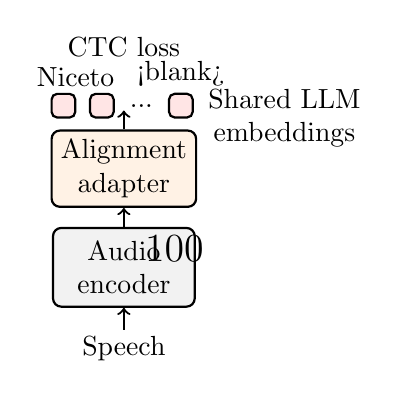
\begin{tikzpicture} [scale=0.8]
        \node(ae) at (0,0) [rectangle, draw=black, fill=gray!10, rounded corners=3pt, thick, minimum width=1.8cm,minimum height=1cm,align=center] {Audio\\encoder};
        \node(freeze) at ([xshift=0.8cm,yshift=0.3cm]ae.center) [rectangle, align=center] {\Large{\ding{100}}};
        \node(fb) at ([yshift=-0.3cm]ae.south) [rectangle, align=center,anchor=north] {Speech};
        \node(aa) at ([yshift=0.3cm]ae.north) [rectangle, draw=black, fill=orange!10, rounded corners=3pt, thick, minimum width=1.8cm,minimum height=0.5cm,align=center,anchor=south] {Alignment\\adapter};
        
        \node(f1) at ([yshift=1.0cm]aa.west) [rectangle, draw=black, fill=red!10, rounded corners=2pt, thick, minimum width=0.3cm, minimum height=0.3cm,align=center,anchor=west] {};
        \node(f2) at ([xshift=0.2cm]f1.east) [rectangle, draw=black, fill=red!10, rounded corners=2pt, thick, minimum width=0.3cm, minimum height=0.3cm,align=center,anchor=west] {};
        \node(f3) at ([xshift=0.075cm]f2.east) [rectangle, draw=white,  thick, align=center,anchor=west] {...};
        \node(f4) at ([xshift=0.075cm]f3.east) [rectangle, draw=black, fill=red!10, rounded corners=2pt, thick, minimum width=0.3cm, minimum height=0.3cm,align=center,anchor=west] {};
        \node(t1) at ([yshift=-0.05cm]f1.north) [rectangle, align=center,anchor=south] {Nice};
        \node(t2) at ([yshift=-0.05cm]f2.north) [rectangle, align=center,anchor=south] {to};
        \node(t4) at ([yshift=-0.05cm]f4.north) [rectangle, align=center,anchor=south] {<blank>};
        \node(se) at ([xshift=0.075cm,yshift=-0.2cm]f4.east) [rectangle, align=center,anchor=west] {Shared LLM\\embeddings};
        \node(ctc) at ([yshift=1.0cm]aa.north) [rectangle, rounded corners=3pt, thick, align=center,anchor=south] {CTC loss};

        
        \draw[->,thick]([yshift=-0.05cm]fb.north)--(ae.south);
        \draw[->,thick](ae.north)--(aa.south);
        \draw[->,thick](aa.north)--([yshift=0.3cm]aa.north);

        
      \end{tikzpicture}
    \end{minipage}
    }
    \subfigure[Shrinking stage]{
    \begin{minipage}[t]{0.45\linewidth}
    \centering
    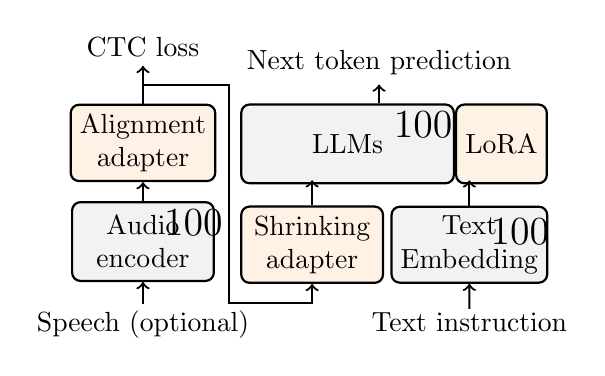
\begin{tikzpicture} [scale=0.8]
        \node(ae) at (0,0) [rectangle, draw=black, fill=gray!10, rounded corners=3pt, thick, minimum width=1.8cm,minimum height=1cm,align=center] {Audio\\encoder};
        \node(freeze) at ([xshift=0.8cm,yshift=0.3cm]ae.center) [rectangle, align=center] {\Large{\ding{100}}};
        \node(fb) at ([yshift=-0.3cm]ae.south) [rectangle, align=center,anchor=north] {Speech (optional)};
        \node(aa) at ([yshift=0.3cm]ae.north) [rectangle, draw=black, fill=orange!10, rounded corners=3pt, thick, minimum width=1.8cm,minimum height=0.5cm,align=center,anchor=south] {Alignment\\adapter};
        \node(ctc) at ([yshift=0.6cm]aa.north) [rectangle,align=center,anchor=south] {CTC loss};
        \node(sa) at ([xshift=0.4cm,yshift=-0.05cm]ae.east) [rectangle, draw=black, fill=orange!10, rounded corners=3pt, thick, minimum width=1.8cm,minimum height=0.5cm,align=center,anchor=west] {Shrinking\\adapter};
        \node(llm) at ([yshift=1.6cm]sa.west) [rectangle, draw=black, fill=gray!10, rounded corners=3pt, thick, minimum width=2.7cm,minimum height=1.0cm,align=center,anchor=west] {LLMs};
        \node(lora) at (llm.east) [rectangle, draw=black, fill=orange!10, rounded corners=3pt, thick, minimum width=1.0cm,minimum height=1.0cm,align=center,anchor=west] {LoRA};
        \node(te) at ([xshift=0.1cm]sa.east) [rectangle, draw=black, fill=gray!10, rounded corners=3pt, thick, minimum width=1.8cm,minimum height=0.5cm,align=center,anchor=west] {Text\\Embedding};
        \node(freeze3) at ([xshift=0.8cm,yshift=0.2cm]te.center) [rectangle, align=center] {\Large{\ding{100}}};
        \node(ti) at ([yshift=-0.3cm]te.south) [rectangle, align=center,anchor=north] {Text instruction};
        \node(freeze2) at ([xshift=1.2cm,yshift=0.3cm]llm.center) [rectangle, align=center] {\Large{\ding{100}}};
        \node(loss) at ([xshift=0.5cm, yshift=0.3cm]llm.north) [rectangle, align=center,anchor=south] {Next token prediction};

        
        \draw[->,thick]([yshift=-0.05cm]fb.north)--(ae.south);
        \draw[->,thick](ae.north)--(aa.south);
        \draw[->,thick](aa.north)--(ctc.south);
        \draw[->,thick](sa.north)--([yshift=0.4cm]sa.north);
        \draw[->,thick](te.north)--([yshift=0.4cm]te.north);
        \draw[->,thick]([yshift=-0.3cm]loss.south)--(loss.south);
        \draw[->,thick]([yshift=-0.1cm]ti.north)--(te.south);

        \draw[->,thick](aa.north)--([yshift=0.3cm]aa.north)--([xshift=0.2cm, yshift=0.3cm]aa.north -| aa.east)--([xshift=0.2cm, yshift=-0.3cm]sa.south -| aa.east)--([yshift=-0.3cm]sa.south)--(sa.south);
      \end{tikzpicture}
    \end{minipage}
    }
    \subfigure[SFT stage]{
    \begin{minipage}[t]{0.20\linewidth}
    \centering
    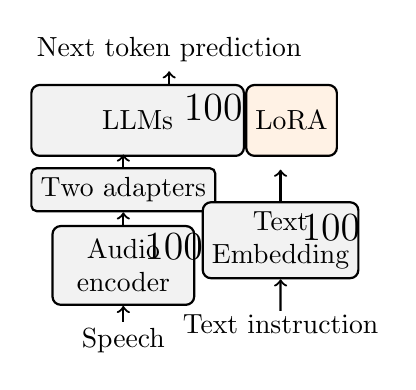
\begin{tikzpicture} [scale=0.8]
        \node(ae) at (0,0) [rectangle, draw=black, fill=gray!10, rounded corners=3pt, thick, minimum width=1.8cm,minimum height=1cm,align=center] {Audio\\encoder};
        \node(freeze) at ([xshift=0.8cm,yshift=0.3cm]ae.center) [rectangle, align=center] {\Large{\ding{100}}};
        \node(fb) at ([yshift=-0.2cm]ae.south) [rectangle, align=center,anchor=north] {Speech};
        \node(aa) at ([yshift=0.2cm]ae.north) [rectangle, draw=black, fill=gray!10, rounded corners=2pt, thick, minimum width=1.8cm,minimum height=0.5cm,align=center,anchor=south] {Two adapters};
        
        \node(llm) at ([yshift=1.1cm]aa.west) [rectangle, draw=black, fill=gray!10, rounded corners=3pt, thick, minimum width=2.7cm,minimum height=0.9cm,align=center,anchor=west] {LLMs};
        \node(lora) at (llm.east) [rectangle, draw=black, fill=orange!10, rounded corners=3pt, thick, minimum width=0.9cm,minimum height=0.9cm,align=center,anchor=west] {LoRA};
        \node(te) at ([xshift=0.1cm,yshift=0.4cm]ae.east) [rectangle, draw=black, fill=gray!10, rounded corners=3pt, thick, minimum width=1.8cm,minimum height=0.5cm,align=center,anchor=west] {Text\\Embedding};
        \node(freeze3) at ([xshift=0.8cm,yshift=0.2cm]te.center) [rectangle, align=center] {\Large{\ding{100}}};
        \node(ti) at ([yshift=-0.4cm]te.south) [rectangle, align=center,anchor=north] {Text instruction};
        \node(freeze2) at ([xshift=1.2cm,yshift=0.2cm]llm.center) [rectangle, align=center] {\Large{\ding{100}}};
        \node(loss) at ([xshift=0.5cm, yshift=0.2cm]llm.north) [rectangle, align=center,anchor=south] {Next token prediction};
       
        \draw[->,thick]([yshift=-0.05cm]fb.north)--(ae.south);
        \draw[->,thick](ae.north)--(aa.south);
        \draw[->,thick](aa.north)--([yshift=0.2cm]aa.north);
        \draw[->,thick](te.north)--([yshift=0.5cm]te.north);
        \draw[->,thick]([yshift=-0.2cm]loss.south)--(loss.south);
        \draw[->,thick]([yshift=-0.1cm]ti.north)--(te.south);
        
      \end{tikzpicture}
    \end{minipage}
    }
      \caption{Training progress of Soundwave. The gray modules are frozen while the orange modules are updated.}
      \label{architecture}
  \end{figure*}

  
